\documentclass[11pt]{exam}

\usepackage{amssymb, amsmath, amsthm, mathrsfs, multicol, graphicx}
\usepackage{tikz}
\usepackage{booktabs}

 \def\d{\displaystyle}
\def\?{\reflectbox{?}}
\def\b#1{\mathbf{#1}}
\def\f#1{\mathfrak #1}
\def\c#1{\mathcal #1}
\def\s#1{\mathscr #1}
\def\r#1{\mathrm{#1}}
\def\N{\mathbb N}
\def\Z{\mathbb Z}
\def\Q{\mathbb Q}
\def\R{\mathbb R}
\def\C{\mathbb C}
\def\F{\mathbb F}
\def\A{\mathbb A}
\def\X{\mathbb X}
\def\E{\mathbb E}
\def\O{\mathbb O}
\def\U{\mathcal U}
\def\pow{\mathcal P}
\def\inv{^{-1}}
\def\nrml{\triangleleft}
\def\st{:}
\def\~{\widetilde}
\def\rem{\mathcal R}
\def\sigalg{$\sigma$-algebra }
\def\Gal{\mbox{Gal}}
\def\iff{\leftrightarrow}
\def\Iff{\Leftrightarrow}
\def\land{\wedge}
\def\And{\bigwedge}
\def\AAnd{\d\bigwedge\mkern-18mu\bigwedge}
\def\Vee{\bigvee}
\def\VVee{\d\Vee\mkern-18mu\Vee}
\def\imp{\rightarrow}
\def\Imp{\Rightarrow}
\def\Fi{\Leftarrow}

%\def\={\equiv}
\def\var{\mbox{var}}
\def\mod{\mbox{Mod}}
\def\Th{\mbox{Th}}
\def\sat{\mbox{Sat}}
\def\con{\mbox{Con}}
\def\bmodels{=\joinrel\mathrel|}
\def\iffmodels{\bmodels\models}
\def\dbland{\bigwedge \!\!\bigwedge}
\def\dom{\mbox{dom}}
\def\rng{\mbox{range}}
\DeclareMathOperator{\wgt}{wgt}


\def\bar{\overline}


\newcommand{\vtx}[2]{node[fill,circle,inner sep=0pt, minimum size=4pt,label=#1:#2]{}}
\newcommand{\va}[1]{\vtx{above}{#1}}
\newcommand{\vb}[1]{\vtx{below}{#1}}
\newcommand{\vr}[1]{\vtx{right}{#1}}
\newcommand{\vl}[1]{\vtx{left}{#1}}
\renewcommand{\v}{\vtx{above}{}}

\def\circleA{(-.5,0) circle (1)}
\def\circleAlabel{(-1.5,.6) node[above]{$A$}}
\def\circleB{(.5,0) circle (1)}
\def\circleBlabel{(1.5,.6) node[above]{$B$}}
\def\circleC{(0,-1) circle (1)}
\def\circleClabel{(.5,-2) node[right]{$C$}}
\def\twosetbox{(-2,-1.4) rectangle (2,1.4)}
\def\threesetbox{(-2.5,-2.4) rectangle (2.5,1.4)}
\newcommand{\twoline}[2]{\begin{pmatrix}#1 \\ #2 \end{pmatrix}}


\def\d{\displaystyle}
\def\?{\reflectbox{?}}
\def\b#1{\mathbf{#1}}
\def\f#1{\mathfrak #1}
\def\c#1{\mathcal #1}
\def\s#1{\mathscr #1}
\def\r#1{\mathrm{#1}}
\def\N{\mathbb N}
\def\Z{\mathbb Z}
\def\Q{\mathbb Q}
\def\R{\mathbb R}
\def\C{\mathbb C}
\def\F{\mathbb F}
\def\A{\mathbb A}
\def\X{\mathbb X}
\def\E{\mathbb E}
\def\O{\mathbb O}
\def\pow{\mathscr P}
\def\inv{^{-1}}
\def\nrml{\triangleleft}
\def\st{:}
\def\~{\widetilde}
\def\rem{\mathcal R}
\def\iff{\leftrightarrow}
\def\Iff{\Leftrightarrow}
\def\and{\wedge}
\def\And{\bigwedge}
\def\Vee{\bigvee}
\def\imp{\rightarrow}
\def\Imp{\Rightarrow}
\def\Fi{\Leftarrow}



\def\circleA{(-.5,0) circle (1)}
\def\circleAlabel{(-1.5,.6) node[above]{$A$}}
\def\circleB{(.5,0) circle (1)}
\def\circleBlabel{(1.5,.6) node[above]{$B$}}
\def\circleC{(0,-1) circle (1)}
\def\circleClabel{(.5,-2) node[right]{$C$}}
\def\twosetbox{(-2,-1.5) rectangle (2,1.5)}
\def\threesetbox{(-2,-2.5) rectangle (2,1.5)}


\def\bar{\overline}

%\pointname{pts}
\pointsinmargin
\marginpointname{pts}
\marginbonuspointname{bns-pts}

\addpoints
\pagestyle{headandfoot}
% \printanswers

\firstpageheader{Math 228}{\bf\large Final Exam}{December 6, 2017}
\runningfooter{}{\thepage}{}
\extrafootheight{-.45 in}



\begin{document}
%space for name
\noindent {\large\bf Name:} \underline{\hspace{2.5 in}}
\vskip 1em

\noindent{\bf Instructions:} Answer each of the following questions.  Answers without supporting work or explanations will be counted as incorrect.  When asked to explain, justify, or prove your answers, use complete English sentences.
% (There are \numquestions\, questions worth \numpoints\, points.)



\begin{questions}

\question[12] Let $A = \{1, 2, 3, \ldots, 100\}$.  You would like to know how many subsets of $A$ contain exactly 5 elements.
\begin{parts}
	\part One of your friends mistakingly thinks the answer should be $P(100,5)$.  Explain why this is wrong by explicitly referencing outcomes your friend is over or under counting.
	\begin{solution}
		This would be $100\cdot 99 \cdot 98 \cdot 97 \cdot 96$.  One of the outcomes that this counts is the set $\{3, 4, 7, 9, 85\}$.  But it also counts $\{9, 85, 3, 4, 7\}$ as a distinct outcome.  These are equal as sets, so your friend is over counting different arrangements of the same set.
	\end{solution}
	 \vfill
	\part How many times larger or smaller is your friend's answer compared to the correct one.  Explain why this makes sense.
	\begin{solution}
		For each subset of $A$ containing 5 elements, your friend is counting $5! = 120$ different arrangements.  Thus your friend's answer is 120 times larger than the correct answer of ${100 \choose 5}$.
	\end{solution}
	 \vfill
	\part Another one of your friends believes you should use stars and bars to answer the question.  Explain why this is wrong, again referencing outcomes.
	\begin{solution}
		Stars and bars would allow for repeated elements in the subset (two stars between a pair of bars).  One of these outcomes would be $\{2, 2, 3, 84, 84\}$.  But that is not a set of size 5 (there are only 3 elements in it).
	\end{solution}
	\vfill

\end{parts}


% \question[9] Timmy has just started going to the gym. He has figured out that there are 20 different machines that he uses on a regular basis. Each visit he selects a \emph{sequence} of 5 different machines to use.
% 	\begin{parts}
% 		\part How many days could Timmy go without having to repeat any workout sequence? Explain.
% 			\begin{solution}
% 					$P(20,5)$
% 			\end{solution}
% 	\vfill
% 		\part Timmy's schedule changed and he now has to go to the gym during peak hours. So this means that he cannot decide on the {\em sequence} ahead of time, only the {\em set} of 5 machines he will use. How many times can he go without having to use the same set? Explain.
% 			\begin{solution}
% 				${ 20 \choose 5}$
% 			\end{solution}
% 	\vfill
% 		\part Explain the relationship between your two answers above using the context of the problem. Don't just say which is bigger, but say how many times bigger it is, and say why this makes sense.
% 			\begin{solution}
% 				Part a is $5!$ times bigger than part b.
% 			\end{solution}
% 		\vfill
% 	\end{parts}


\newpage


\question[12] Answer each of the relatively simple counting questions on this page.  No explanation is needed, but a very short indication of your reasoning might get you some partial credit.

\begin{parts}
	\part How many different bags of 20 Skittles are possible, assuming we care about how many of each of the 5 ``flavors'' are in the bag?
	\begin{solution}
		${24 \choose 4}$. Stars and bars with 20 stars and 4 bars.
	\end{solution}
	\vfill
	\part How many stacks of 9 coins are possible, using pennies, nickels, dimes, and quarters?
	\begin{solution}
		$4^9$.  You can choose one of 4 coin types in each of the 9 positions.
	\end{solution}
	\vfill
	\part How many bit strings of length 12 have weight either 5 or 6?
	\begin{solution}
		${12 \choose 5} + {12 \choose 6}$ (there is no way for a bit string to have both).
	\end{solution}
	\vfill
	\part How many \emph{injective} (one-to-one) functions have domain $\{1,2,3,4,5\}$ and codomain $\{a, b, c, d, e, f, g\}$?
	\begin{solution}
		$P(7,5) = 7 \cdot 6 \cdot \cdots \cdot 3$.  Each element in the domain has 7 possible images, but can't repeat any.
	\end{solution}
	\vfill
	\part How many edges does $K_{17}$ have?
	\begin{solution}
		${17 \choose 2}$, which is the same as $\frac{17 \cdot 16}{2} = 136$.
	\end{solution}
	\vfill
	\part How many ways are there to divide 15 students into three groups of 5?
	\begin{solution}
		${15 \choose 5}{10 \choose 5}{5 \choose 5}$
	\end{solution}
	\vfill

\end{parts}




% %REPHRASE NEXT TIME. Underline key words, or insist they give an answer to part c somewhere.  Lots of students also did not explain why the answers allowed for repeats in terms of the answer, but in terms of the problem statement :(.
% \question[12] Suppose you own a large collection of magnetic alphabet letters that you keep in a basket next to your fridge. You like to spell out encouraging messages on your fridge every morning, so you have plenty of each of the 26 letters of the alphabet.
% %\begin{choices}
% %\begin{multicols}{4}
% %\choice $ P(10,6)$
% %\choice ${10 \choose 6}$
% %\choice $10^6$
% %\choice ${15 \choose 9}$
% %\end{multicols}
% %\end{choices}
%
% \begin{parts}
%  \part How many different 8 letter ``words'' can you make on your fridge?
% \begin{solution}
% 	$26^8$
% \end{solution}
%  \vfill
%  \part Does the answer you gave above allow for repeated letters? Explain why, incorporating what your answer would have been if you did not assume what you did.
%
% \begin{solution}
% 	Yes, part a did assume repeated letters were allowed. Explanation needs to incorporate a permutation 	$P(26,8)$.
% \end{solution}
%
%  \vfill
% % \part How many handfuls of 8 can you grab out of the basket?
% % \vfill
% % \part In the answer you gave above, did you assume repeated letters were allowed? Explain why incorporating what your answer would have been if you did not assume what you did.
% % \vfill
%
% 	\part Explain why stars and bars are not helpful for either of the above two parts. Write a question using the context of magnetic letters that is solvable using stars and bars.
% 		\begin{solution}
% 		Stars and bars allows for repeated letters, but does not distinguish between different orders of those letters.  It could be used to answer the question: how many handfuls for 8 letters could you grab out of the collection.  The answer would use 8 stars and 25 bars, so ${33 \choose 8}$.
% 		\end{solution}
%
%
% \vfill
% 	\part Explain why your question in part (c) allows for repeated letters. What would the answer be if your question did not involve repeats.
% 		\begin{solution}
% 			Since you can have two stars next to each other (not separated by a bar), you can have that letter repeated.  The number of 8-letter handfuls not containing repeated letters is ${26 \choose 8}$.
% 		\end{solution}
% \vfill
% \end{parts}

\newpage


\question[9] Suppose you had 8 identical bow ties to give away as gifts to your 3 favorite math professors.

\begin{parts}
	\part Describe a particular outcome and show how to represent it using a string of two types of symbols.
	\begin{solution}
		You could give 5 ties to the first prof, none to the second, and 3 to the third.  This would be represented using a stars and bars diagram as
		\[*****||***\]
	\end{solution}
	\vfill
	\part Find the number of ways to distribute the 8 bow ties to the 3 professors.
\begin{solution}
 Each outcome is represented by a string of 8 stars and 2 bars.  Thus there are ${10 \choose 8}$ outcomes.
\end{solution}
	\vfill

	\part What if the 8 bow ties were all different colors.  Now how many ways are there to distribute them to the 3 professors?  Explain.
\begin{solution}
	This is like counting the number of functions from a set of size 8 to a set of size 3.  There are three choices for each bow tie, so there are $3^8$ ways to distribute the ties.
\end{solution}
\vfill


\end{parts}






\question[4] How many lattice paths starting at $(0,0)$ end at $(10,10)$ and pass through $(2,4)$ or $(6,7)$ (or both)?  Explain your answer.

Note: if you consider three cases, make sure you say how to combine those cases to arrive at your single correct answer.
\begin{solution}
	${6 \choose 2}{14 \choose 8}+{13\choose 6}{7 \choose 4} - {6 \choose 2}{7 \choose 4}{7 \choose 4}$
\end{solution}
\vfill
\vfill

\newpage

\question Consider the sequence $(a_n)_{n\ge 0}$, which begins $1,5,13,41,121,\ldots$, defined by $a_n = 2a_{n-1} + 3a_{n-2}$ with $a_0 = 1$, $a_1 = 5$.
\begin{parts}
 	\part[5] Find a closed formula for the sequence.
	\begin{solution}
	$a_n = \frac{3}{2}3^n - \frac{1}{2}(-1)^n$.
	\end{solution}
 	\vfill
	\vfill
% 	\part[4] Find the generating function for the sequence.
% 	\vfill
 	\part[3] Will the $n$th differences (i.e., differences, or differences of differences, etc) of the sequence ever be constant?  Explain.
 	\begin{solution}
 	No, because if they were, then the closed formula would be a polynomial.
 	\end{solution}
 	\vfill
\end{parts}



\question[5] Find a closed formula for the sequence $(b_n)_{n \ge 1}$ which begins $4, 11, 21, 34, 50, 69, \ldots$ (note $4 = b_1$).
	\begin{solution}

	\[b_n = \frac{(3n+5)n}{2}\]

	\end{solution}
	\vfill
	\vfill


\newpage


\question[4] Make a truth table for $(B\vee C) \imp \neg H$

\begin{center}
  \begin{tabular}{c|c|c||c}

  $B$ & $C$ & $H$ & \hspace{5 in} \\ \hline & & & \\
  T & T & T & \\ & & & \\
  T & T & F & \\ & & & \\
  T & F & T & \\ & & & \\
  T & F & F & \\ & & & \\
  F & T & T & \\ & & & \\
  F & T & F & \\ & & & \\
  F & F & T & \\ & & & \\
  F & F & F & \\
  \end{tabular}
\end{center}

  \begin{solution}

  \begin{tabular}{c|c|c||c}

    $B$ & $C$ & $H$ & $(B\vee C) \imp \neg H $ \\ \hline
    T & T & T & F\\
    T & T & F & T\\
    T & F & T & F\\
    T & F & F & T\\
    F & T & T & F\\
    F & T & F & T\\
    F & F & T & T\\
    F & F & F & T\\
    \end{tabular}

  \end{solution}
Consider the statement about graphs: ``If a graph is bipartite or complete, then it is not Hamiltonian'' (you do not need to know what Hamiltonian means to complete this problem).

\begin{parts}
\part[3] If you wanted to prove the statement \emph{false}, what properties would a counterexample graph need to possess?  Explain.  You must reference your truth table to receive credit.
\begin{solution}
We would need to be in rows 1, 3, or 5.  So for example, we could find a graph that was bipartite, complete and Hamiltonian.  In particular, we must have a graph that is Hamiltonian, and have that it is either bipartite, complete, or both.
\end{solution}
\vfill
\part[3] If the statement were \emph{true} and you had a graph that \emph{was} Hamiltonian, what could you conclude about that graph?  Explain, again \textbf{using the truth table}.
\begin{solution}
How $H$ is true, as well as the whole statement.  We must be in row 7 of the table, so we know that $B$ and $C$ are both false.  Thus the graph is not bipartite and not complete.
\end{solution}
\vfill
\end{parts}


\newpage



\question Consider the statement, ``If two graphs are isomorphic, then they have the same chromatic number.''
\begin{parts}
	\part[2] Write the converse of the statement.
	\vfill
	\part[2] Write the contrapositive of the (original) statement.
	\vfill
	\part[2] If you wanted to prove the original statement by contradiction, what would your initial assumption be?  That is, write the first line of such a proof.
	\vfill
	\part[4] In fact, the original statement is true.  \underline{Use this} to prove that the following two graphs are NOT isomorphic.  You should draw out the graphs as a first step.
	\[G_1: V_1 = \{a,b,c,d,e\}, E_1 = \{ab, ac, ad, ae, bc, cd, de\} \]
	\[G2: V_1 = \{u, v, w, x, y\}, E_2 = \{uv, uw, ux, vw, vx, wx, wy\}\]
	\vfill
	\vfill
	\vfill
	\part[4] Prove that the converse of the original statement is false by giving a counterexample.
	\vfill
	\vfill
	\vfill
\end{parts}

% \question[12] Consider the statement about graphs with $n$ vertices, ``if some vertex is not adjacent to all other vertices, then the graph has fewer than ${n \choose 2}$ edges.''    Note that we can say vertices $x$ and $y$ are not adjacent in symbols by writing $\{x,y\} \notin E$.
%
% \begin{parts}
% \part Write the converse of the statement (in words)
% \begin{solution}
% If the graph has fewer than ${n \choose 2}$ edges, then there is some vertex not adjacent to all other vertices.
% \end{solution}
%
% \vfill
%
% \part Write the contrapositive of the statement (in words).
% \begin{solution}
% If the graph has at least ${n\choose 2}$ edges, then every vertex is adjacent to at least one other vertex.
% \end{solution}
% \vfill
%
% \part Write the negation of the statement (in words).
% \begin{solution}
% There is some vertex not adjacent to all other vertices, and the graph has at least ${n \choose 2}$ edges.
% \end{solution}
%
%
% \vfill
%
% \part Label the statements written in symbols below as the original (the statement above), converse, contrapositive, negation or none of the above.
% \vskip 2em
% $|E| \ge {n \choose 2} \imp \forall x \exists y (x \ne y  \wedge \{x,y\} \in E)$
% \begin{solution}
% Contrapositive.
% \end{solution}
% \vskip 2em
% $\exists x \forall y (x \ne y \imp \{x,y\} \notin E) \imp |E| < {n \choose 2}$
% \begin{solution}
% Original.
% \end{solution}
% \vskip 2em
% $\forall x \exists y (x = y \imp {x,y} \in E) \imp |E| \ge {n \choose 2}$
% \begin{solution}
% None.
% \end{solution}
% \vskip 2em
% $|E| < {n \choose 2} \imp \exists x \forall y (x \ne y \imp \{x,y\} \notin E)$
% \begin{solution}
% Converse.
% \end{solution}
% \vskip 2em
% $\exists x \forall y (x \ne y \imp {x,y} \notin E) \wedge |E| \ge {n \choose 2}$
% \begin{solution}
% Negation.
% \end{solution}
% \vskip 2em
%
% \part Is the original statement true or false?  Explain.  (You will need to use knowledge of graph theory and counting to answer this).
% \begin{solution}
% True.  If there is a vertex not adjacent to anything else, then the graph is not complete.  A complete graph has ${n \choose 2}$ edges, so our graph will have fewer than this.
% \end{solution}
% \vfill
% \end{parts}

%
%\question[6] Consider the statement $\forall x (x>0\imp \exists y (0<y\wedge y<x))$.
%\begin{parts}
%	\part Write the converse of the statement.
%	\begin{solution}
%	$\forall x (\exists y (0<y \wedge y < x) \imp x> 0)$
%
%	\end{solution}
%	\vfill
%	\part Write the contrapositive of the statement.
%	\begin{solution}
%	$\forall x (\forall y (0 \ge y \vee y \ge x) \imp x \le 0)$
%	\end{solution}
%	\vfill
%	\part Write the negation of the statement.
%	\begin{solution}
%	$\exists x (x > 0 \wedge \forall y (0\ge y \vee y \ge x))$
%	\end{solution}
%	\vfill
%\end{parts}
%\question[6] Consider the statement ``If a number is positive then there is a positive number less than it.''
%\begin{parts}
%	\part Write the converse of the statement.
%	\begin{solution}
%	If there is a positive number less than a number, then it is positive.
%	\end{solution}
%	\vfill
%	\part Write the contrapositive of the statement.
%	\begin{solution}
%	If there is not a positive number less than a number, then it is not positive.
%	\end{solution}
%	\vfill
%	\part Write the negation of the statement.
%	\begin{solution}
%	There is a number which is positive but there is no positive number less than it.
%	\end{solution}
%	\vfill
%\end{parts}
%\question[2] Jack thinks that the original statements from the above questions are true, but Jill thinks they are both false. Explain how they could both be correct.
%\begin{solution}
%It depends what set they are quantifying over.  If we are talking about the integers, the statement is false (there is no positive number less than 1).  If we are talking about the real numbers, you can always divide the positive number by 2 and get a smaller positive number.
%\end{solution}
%\vfill
%\vfill
%\vfill

%\question[5] The Four Color Theorem says: ``if a graph is planar, then the chromatic number is at most 4.''
%Which of the following statements are logically equivalent to the theorem?
%\begin{parts}
%	\part The set of planar graphs is a subset of the set of graphs which have chromatic number at most 4.
%	\vfill
%	\part The set of planar graph is equal to the set of graphs with chromatic number at most 4.
%	\vfill
%	\part For any graph $G$, if $G$ is not planar, then $G$ has chromatic number greater than 4.
%	\vfill
%	\part It is necessary for a graph to have chromatic number at most 4 in order for it to be planar.
%	\vfill
%%	\part To have chromatic number at most 4, it is sufficient for the graph to be planar.
%%	\vfill
%	\part Either a graph is planar or has chromatic number greater than 4.
%	\vfill
%\end{parts}
\newpage

\question A graph is called {\em $k$-regular} if every vertex has degree $k$.
\begin{parts}
	\part[4] Explain why any $k$-regular graph with 11 vertices must contain an Euler circuit.\\  (Hint: what can you say about the possible values of $k$?)
	\begin{solution}
	The graph will have $11k/2$ edges, so $k$ must be even.  But if every vertex has even degree, there is an Euler circuit in the graph.
	\end{solution}
	\vfill
	\part[4] Suppose $G$ is an $6$-regular graph. Must the chromatic number of $G$ be at least 6?  Explain.
	\begin{solution}
	No.  We could have a bipartite graph which was $6$-regular.  For example, $K_{6,6}$.  This has chromatic number 2.
	\end{solution}
	\vfill
	\part[6] Prove that any $6$-regular graph with 11 vertices must NOT be planar.  State the style of proof you are using.
	\begin{solution}
	Such a graph would have 33 edges, and if it were planar, would have $F = 2 - 11 + 33 = 24$ faces.  But any graph satisfies $3f \le 2e$ because each face is surrounded by at least 3 edges, counting each edge for two faces.  This would say that $72 \le 66$ which is a contradiction.
	\end{solution}
	\vfill
	\vfill
\end{parts}




\newpage

\question Each day you cut off one leaf of your tree, but each remaining leaf sprouts two more:

\begin{center}
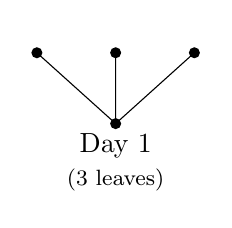
\begin{tikzpicture}[yscale=.9]
\coordinate (a1) at (0,0);
\coordinate (b1) at (-1,1);
\coordinate (b2) at (0,1);
\coordinate (b3) at (1,1);
\draw (a1) \v -- (b1) \v (a1) -- (b2) \v (a1) -- (b3) \v;
\draw (0,0) node[below]{Day 1} (0,-.5) node[below]{\footnotesize(3 leaves)};
\end{tikzpicture}
\hfill
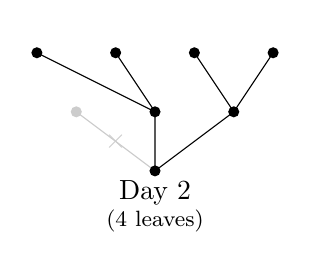
\begin{tikzpicture}[yscale=.75]
\coordinate (a1) at (0,0);
\coordinate (b2) at (-1,1);
\coordinate (b1) at (0,1);
\coordinate (b3) at (1,1);
\coordinate (c1) at (-1.5,2);
\coordinate (c2) at (-.5, 2);
\coordinate (c3) at (.5, 2);
\coordinate (c4) at (1.5,2);
\draw[black!20!white] (a1) -- (b2) \v (a1) (-.5,.5) node{$\times$};
\draw (a1) \v -- (b1) \v -- (c1) \v (b1) -- (c2) \v (a1) -- (b3) \v -- (c3) \v (b3) -- (c4) \v;
\draw (0,0) node[below]{Day 2} (0,-.5) node[below]{\footnotesize(4 leaves)};
\end{tikzpicture}
\hfill
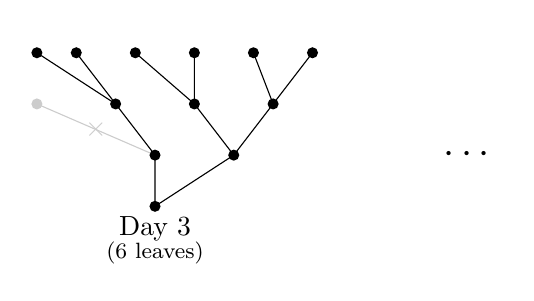
\begin{tikzpicture}[yscale=.65]
\coordinate (a1) at (0,0);
\coordinate (b2) at (-1,1);
\coordinate (b1) at (0,1);
\coordinate (b3) at (1,1);
\coordinate (c1) at (-1.5,2);
\coordinate (c2) at (-.5, 2);
\coordinate (c3) at (.5, 2);
\coordinate (c4) at (1.5,2);
\coordinate (d1) at (-1.5, 3);
\coordinate (d2) at (-1, 3);
\coordinate (d3) at (-.25, 3);
\coordinate (d4) at (.5,3);
\coordinate (d5) at (1.25,3);
\coordinate (d6) at (2,3);
\draw[black!20!white] (b1) -- (c1) \v (-.75,1.5) node{$\times$};
\draw (a1) \v -- (b1) \v (b1) -- (c2) \v (a1) -- (b3) \v -- (c3) \v (b3) -- (c4) \v;
\draw (c2) -- (d1) \v (c2) -- (d2) \v (c3) -- (d3) \v (c3) -- (d4) \v (c4) -- (d5) \v (c4) -- (d6) \v;
\draw (0,0) node[below]{Day 3} (0,-.5) node[below]{\footnotesize(6 leaves)};
\draw (4,1) node{\Large $\cdots$};
\end{tikzpicture}
% \hfill $\cdots$
\end{center}
\begin{parts}
	\part[3] How many \textbf{leaves} (vertices with degree 1) will your tree have on day 6?  Show your work.
	\begin{solution}
	The sequence is $3,4, 6, 10, 18, 34,\ldots$ so on day $6$ you have 34 leaves.
	\end{solution}
\vfill
	\part[3] Let $L_n$ denote the number of \textbf{leaves} your tree has on day $n$.  Find a \emph{recursive} definition for $L_n$ and explain why your answer makes sense.
	\begin{solution}
	Each day you cut off one of the leaves, and then for each remaining leaf you get two leaves.  So
	\[L_n = 2(L_{n-1} - 1) = 2L_{n-2} - 2\]
	\end{solution}
\vfill
	\part[6] Prove, using mathematical induction, that $L_n < 2^n$ for all $n > 2$. Make sure that you are explicit about the format of the proof!
	\begin{solution}
	Let $P(n)$ be the statement, ``$L_n < 2^n$.''  We will show that $P(n)$ is true for all $n > 3$.

	Base case: $L_3 = 6 < 8 = 2^3$.

	Inductive case: Assume $P(k)$ is true for an arbitrary $k > 3$.  That is $L_k < 2^k$.  Consider $L_{k+1}$.  We can get $L_{k+1}$ from $L_k$ by doubling it and subtracting 2.  But we can get $2^{k+1}$ from $2^k$ by just doubling it.  So if $L_k$ is already smaller than $2^k$, $L_{k+1}$ will be smaller than $2^{k+1}$.  Formally, we can see this as follows:
	\begin{align*}
	L_k & < 2^k \\
	2L_k & < 2^{k+1} \\
	2L_k - 2 &< 2^{k+1}\\
	L_{k+1} < 2^{k+1}
	\end{align*}
	So $P(k+1)$ is true as well.

	Therefore, by the principle of mathematical induction, $P(n)$ is true for all $n > 2$.
	\end{solution}
\vfill
\vfill
\vfill


\end{parts}

% \newpage


% \bonusquestion[10] BONUS!! For the sequence of trees in the last problem, give both recursive and closed formulas for $E_n$, the number of \emph{edges} in the tree on day $n$.  For full credit, you must explain how you know the two formulas are correct.
%
% \begin{solution}
% The sequence for the number of edges on day $n$ is $3, 6, 11, 20, 37,\ldots$.  A recursive formula for $E_n$ is
% \[E_n = 3E_{n-1} - 2E_{n-2} - 1\]
% You can see this is correct by considering how many new edges appear each day.  You get two new edges for each of all but one of the new edges the day before.  The new edges from yesterday is $E_{n-1} - (E_{n-2}-1)$ (the edges yesterday less the edges already there the day before that), so if we subtract 1 from this and then double the result we will get the number of new edges today:
% \[2(E_{n-1} - (E_{n-2}-1)-1) = 2E_{n-1} - 2E_{n-2}\]
% To get the total number of edges, we add this to $E_{n-1}$, the number of edges yesterday, and subtract one for the one we cut off.
%
% To get a closed formula, note that the number of edges is roughly doubling each day. So compare the sequence to the powers of 2.  If you do this, you see that we are off by $n$ on day $n$, so we guess
% \[E_n = 2^n + n\]
%
% To prove this is correct, we show (using induction) that this formula satisfies the recurrence relation.  On day $1$, we have $E_1 = 2^1 + 1 = 3$ as required.  If we assume the formula is correct for all $k < n$, then consider
% \[E_n = 3E_{n-1} - 2E_{n-2} - 1 = 3(2^{n-1} + n-1) - 2(2^{n-2} + n - 2) - 1 = 3\cdot 2^{n-1} + 2 2^{n-2} + n = 2^n + n\]
% as required.
%
% \end{solution}
\end{questions}




\end{document}
